\chapter{Techniques for Updating and Synchronising Geodata} \label{chap:tech}
When submission of new data and modifications on existing data is done for the cadastre and basic map data in Norway, one of the criteria is that all the databases with the same content are updated regardless of where the update is done. What is needed is a geosynchronization service. The synchronization of FKB data is done with \textit{geosynchronisation}, the updating is done through the \textit{NGIS-API}, while the cadastre data is done through the \textit{MatrikkelAPIs}.  This chapter deals with these three techniques,as well as web services, for getting access to and synchronizing geospatial data.  


\section{Quadri Map Server (QMS) and Its Synchronising Services}\label{ngis}
The \textit{Quadri Map Server} (QMS) is the server of the SFKB system,
%To synchronize, update or upload data onto the QMS server, either the \textit{NGIS-API} or \textit{geosynchronisation} is used \citep{Kartverket2017}. 
and has a client-server architecture. That is, the servers distribute the data while the clients are able to both fetch and perform services on them \citep{NorkartAS2010}. 
%The NGIS-API is an application programming interface for storing spatial data, and GeoSynkronisering is a standard for synchronizing spatial data across different platforms and system solutions \citep{Kartverket2017, Kartverket2013}.
The structure of the QMS system
%with the NGIS-API
is depicted in Figure \ref{fig:qmsfig}. The \textit{archives} (data stores) are used for storing the FKB-data, the \textit{portals} define the clients and authorize users for different tasks, where a task is defined as access to an archive. The data stored in, and uploaded into, QMS is defined by the \textit{object catalogue}, and the service of translating logical, humanly meaningful, names of the distributing servers is the \textit{name server}. All the feature instances in the archives are given unique identifiers. The attributes of the identifiers are LocalId, VersionId and Namespace. Namespace is identifying the data source of the instance, the VersionId identifies the version of the object and the LocalId, based on a Universally unique identifier (UUID), ensures that each feature instance is unique\footnote{The probability to get the same number is small because there are som many possibilities. E.g., the number of random version 4 UUIDs which need to be generated in order to have a 50\% probability of at least one collision, is 2.71 quintillion. This is computed as follows: $ n \approx \frac{1}{2} + \sqrt{\frac{1}{4}+2 \times \ln{2} \times  2^{122}} \approx 2.71 \times 10^{18} $ \citep{Eggan2017}}. 
The \textit{NGIS-API} is the application programming interface for storing spatial data into QMS. \todo{skal jeg flytte denne setningen opp til over identifikatorene?}
.

\begin{figure}[H]
	\centering
	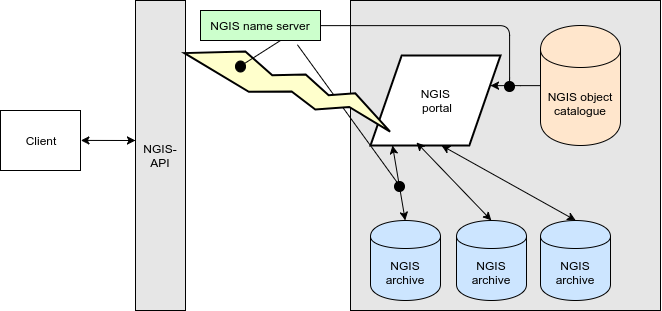
\includegraphics[scale=0.5]{img/ngiss.png}
	\caption{The structure of the Quadri Map Server (QMS) system. For updating the data in QMS the NGIS-API is used.  The main components of the system are portals, object catalogue and archives. It is possible to use geosynchronisation (chapter \ref{geosync}) to manage the data in QMS, in addition to the NGIS-API. Figure adapted from \citep{Kartverket2017b} }
	\label{fig:qmsfig}
\end{figure}

\subsection{NGIS-API}

When editing an existing object, say a building or the land use of an area, in QMS, the object gets locked in the archive, and the user edits the object locally. When the updating is done, the user has to send the object, along with objects that have been edited, added or deleted, back to its archive. When the objects are locked in the archives, other users cannot edit the same object, but they might look at it. This process is called \textit{long transactions} \citep{Kartverket2017b}.



%The service of translating logical, humanly meaningful, names of the distributing servers into unique identifiers (UUID) is the Name server. The Name server is a computer permanently connected to the Internet and is invisible to the common client of the QMS system. Because the servers are registered in the Name server at initialization, starting a server on a new machine will automatically update the Name server. 

%\subsection{Portals}
%It is the portals that handles the client access to the data in QMS, and the clients and their available tasks are defined here. A client's task is for updating and reading into QMS via teh NGIS-API

%The archives 
%\begin{itemize}
%	\item navnetjeneste
%	\item portaler
%	\item archives
%	\item object catalogues.
%\end{itemize}



\subsection{\textit{GeoSynkronisering} - the Geosynchronisation Standard}\label{geosync}

Geosynchronising (\textit{GeoSynkronisering}) is a Norwegian standard for synchronising geographical information across computer systems, and is a provider-subscriber system as illustrated in figure \ref{fig:geosync}. The \textit{provider} updates the database with new data, while the \textit{subscribers} are allowed to update their databases with the changes done by the provider. The SFKB works as a provider: if data is changed or added in QMS, the features will automaticly be geosynchronised to all subscribers. Common subscribers in the SFKB-system are the municipalities and GeoNorge. GeoNorge is the web page where public agencies and institutions, as well as private actors, can get map data and other geospatial information for Norway.  
\\
\begin{figure}[H]
	\centering
	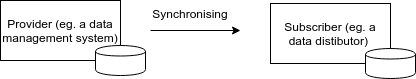
\includegraphics[scale=0.6]{img/geosync.png}
	\caption{The geosynchronisation concept, adopted from \cite[p.~16]{Kartverket2013}. }
	\label{fig:geosync}
\end{figure}


The project of making a standard interface for geosynchronisation services in Norway was carried out in 2012, and was a collaboration between Kartverket, the Norwegian Institute of Bioeconomy Research (NIBIO) and system providers in Norway. Geosynkronisering is a open and freely available project on GitHub, and this Norwegian standard is based on the concepts and methods from international standards, i.e. ISO 19100 Geographic Information/Geomatics and Open Geospatial Consortium (OGC) \citep{Eggan2017,Kartverket2013}.

The geosynchornisation standard is model driven, using models as key artefacts in the development.
%describing the data of an application or domain
UML is used on the conceptual level to describe the data, and on the the data format with GML, using XSD as an application schema showing the meta data. An example of a UML is given below.

\begin{figure}[H]
	\centering
	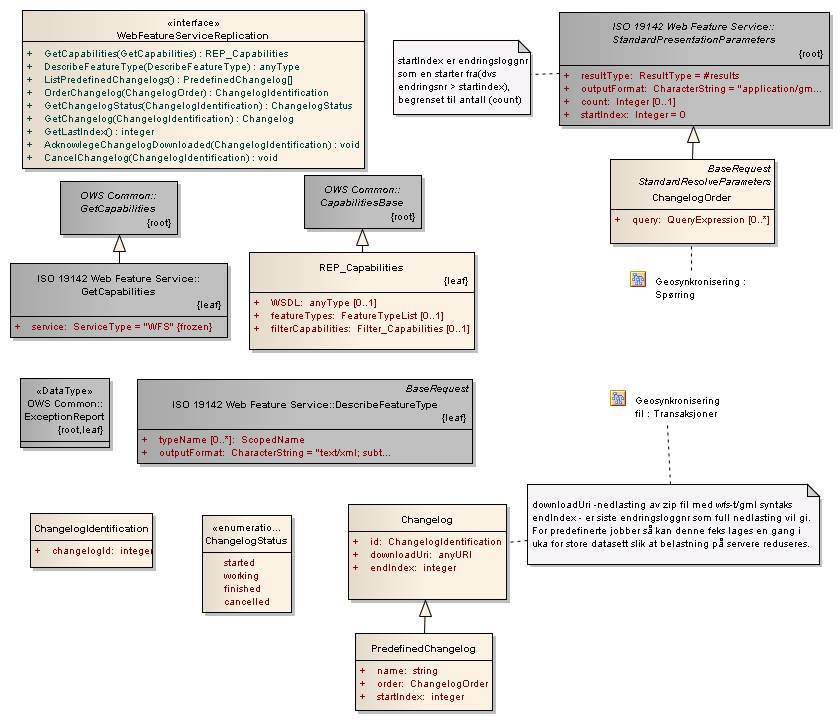
\includegraphics[scale=0.35]{img/uml.png}
	\caption{Figure from \cite{Kartverket2012a} showing an UML model of the services of the geosynchronisation.}
	\label{fig:uml}
\end{figure}

The data transfer with geosynchronising (figure \ref{fig:geosyncprocess}) is a set of transactions of changed features on the GML-format and their respective changelogs are specified by the WFS-T.  GML (Geography Markup Language) is an open interchange format for geographic transactions and a modelling language for geospatial systems \citep{OGC2017}. WFS-T (Transactional Web Feature Service) allows creation, deletion, and updating of geospatial features on the web \citep{OGCNetwork} and will be further described in chapter \ref{wfs}. 

\begin{figure}[H]
	\centering
	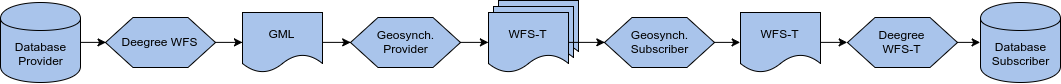
\includegraphics[scale=0.43]{img/geosynkkk.png}
	\caption{A detailed description of the Norwegian geosynchronisation process, adapted from \cite{Eggan2017}. The data stored in the database TODO . Deegree is an implementation of the Web Feature Service}
	\label{fig:geosyncprocess}
\end{figure}



%TODO Sjekk ut dette og fyll det ut: For the SFKB system the municipalities, and the other agencies managing the updating of the FKB data in Norway, will still have a local copy of the geodata. It is this copy they are editing  \citep{Kartverket2016}  
\section{The Central Cadastral Server and its APIs}
%There are several services provided by the cadastre;  The cadastral server has the logic for managing and assembling the cadastral records), as well as control and validation of the business rules of the information. Clients of the cadastre can update and read the cadastal records through the MatrikkelAPI \citep{Difi2014, Matrikkelavdelingen2017}. 
%(a further presentation of the MatrikkelAPI and system will be provided in chapter \ref{chap:matrikkelapi})
%As was stated in chapter ref 
There are several services provided by the cadastre, Matrikkelen; the \textit{cadastral server} serves all clients, both editing and viewing (figure \ref{fig:matr}). The logic of the cadastre server includes management and assembling of cadastre information, as well as control and validation of the business rules of it. The only way to get access to the data on the \textit{cadastre database} is through the \textit{MatrikkelAPI} (chapter \ref{matrikkelapi}) that is on the cadastral central server \citep[p.~338]{Matrikkelavdelingen2017}. Submissions and modifications on the cadastral data are done to the centralised data store directly, as for the new SFKB system. When wanting to keep a local cadastre copy, the Matrikkel system provides a \textit{Changelog API} for synchronizing changes on the central data store. See figure \ref{fig:matr}. 

The physical architecture of the central cadastral server is clustered, meaning there are several physical servers, but for the clients they will appear as one. %(High-Availability Cluster? \citep{IWebTechnologies2015})


\subsection{The MatrikkelAPIs} \label{matrikkelapi}
The MatrikkelAPIs is application programming interfaces for extracting data, in both small and large scale, of the cadastral data.  

There are three MatrikkelAPIs. The first one is for the clients with access to updating the cadastre data - the \textit{Editing API}, the second one the \textit{Viewer API} includes services for inspecting and reading the data and the \textit{Changelog API}, as stated earlier, provides services for fetching data changes - primarily for the local copies at the municipalities, but also for external registers.  The Viewing API support other services as well: web services as WMS that deliver georeferenced raster maps
%with addresses as points and buildings and areas for land parcels 
as well as WFS delivering vectorised map	and properties for addresses, buildings and land parcels. 

There are several types of clients to the cadastre system: the \textit{updating}-, \textit{viewing}- and \textit{retrieval clients} as well as \textit{other systems}. The updating clients support inspection and updating for all information on the cadastre, the viewing clients supports inspection of the data, as well as viewing the cadastral data joint with data from external systems, and lastly the retrieval clients supports updating external municipality registers. Other systems using the cadastre system are mainly systems that uses cadastral information for other software solutions, e.g. a municipal specialized system \citep[p.~337-338]{Matrikkelavdelingen2017}.
 
%As for the SFKB system, the municipalities updates the cadastre data directly into a national and centralized database. 

\begin{figure}[H]
	\centering
	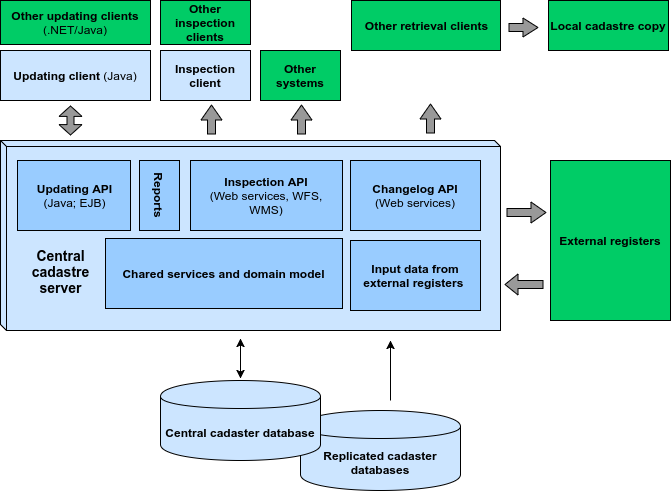
\includegraphics[scale=0.5]{img/matrikkelSYS}
	\caption{The cadastre system, \textit{Matrikkelen}. Solutions for databases through API, clients and relations to other information systems. Adapted from \citep[p.~337]{Matrikkelavdelingen2017} }
	\label{fig:matr}
\end{figure}

\section{Other Generic Services}
There are several web services, ways to access web-based geospatial data. These technologies have been created to facilitate the exchange of geospatial information and to find new ways to communicate geodata and to redefine the work flow of the geospatial analysis. In the following subchapters some of them are presented.  

\subsection{Standard Spesifications from the Open Geospatial Consortium)}\label{OGC}
To get a higher interoperability in the Geographical Information System (GIS) community the Open Geospatial Consortium (OGC) has created standard specifications for data sharing, processing, retrieval, visualisation, content and cataloguing \citep{giuliani2013}.

\subsubsection{The Web Feature Service (WFS)}\label{wfs}

The Web Feature Service (WFS) is a standard geodata extracting service for describing data manipulation on feature level \citep{Peng2005, Norgedigitalt2014}. The specification defines interfaces required to support transactions and query operations on geospatial features over the internet.

The GML-format is the defacto standard transferring format, but WFS supports other formats as well \citep{Eggan2017}. By using GML for the exhange of geospatial data,  interoperability between the heterogeneous system is provided \citep{YaoXiaobai2008Iimo}.

Whereas WFS allows queering and retrieval of features, transactional Web Feature Service (WFS-T) permits the user to create, delete and update features \citep{OGCNetwork},

\subsubsection{The Web Mapping Service (WMS)}
The Web Mapping Service (WMS) is another standad from OGS for exchanging geograpichal information over the web. When using the Web Mapping Service(WMS) the user is given an image of a map that cannot be edited or spatially analysed. 	


\subsection{Simple Object Access Protocol (SOAP)}
Simple Object Access Protocol (SOAP) is a protocol that defines how XML and HTTP are used to get access to objects, services and servers from a web based service, thus aiding in interoperability. SOAP defines an envelope for Web Service messages, where the envelope consists of a header with meta data, e.g. how the recipient of the SOAP message should interpret the message, and the body with the actual message. SOAP is often referred to as Web Service, as it is the original web service \citep{Kartverket2013}, and may serve as a standard for all systems, because it is platform independent \citep{Sipes2004}. 

The Cadastre Viewing and Changelog APIs and the geosynchonisation are examples of SOAP web services. 
%Tjenestegrensesnitt med mekanismer for å hente ut objekter fra en web-basert tjeneste. Ofte omtalt som Web Service (den opprinnelige web servicen). 


\subsection{Representational State Transfer (REST)}
The definitions of Representational State Transfer (REST) are many \citep{Fielding, Richardson}, this paper uses the description by \cite{Fieldinga}: \textit{REST is a coordinated set of architectural constraints that attempts to minimize latency and network communication while at the same time maximizing the independence and scalability of component implementations}. 
%\cite{Battle2008}: \textit{REST is a pattern of resource operations that has emerged as a de facto standard for service design in Web 2.0 applications.} 

REST is commonly based on the HTTP and HTML standards, and provide simplified calls to services through HTTP. It is only data structures and the transferring of their state that is dealt with in a RESTful service \cite{Battle2008}. The state transferring calls are POST, GET, PUT and DELETE, which receptively creates, reads, updates and deletes resources in the RESTful service. A resource is identified and resolved with a URL.

\begin{figure}[H]
	\centering
	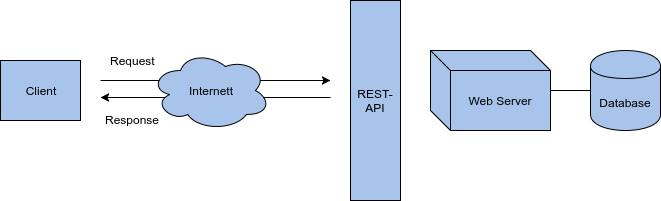
\includegraphics[scale=0.5]{img/REST}
	\caption{REST-API: Clients use  HTTP (or other protocols') queries to create, read, update and delete data on the server-side applications.  Adapted from \citep{Ceeb2013} }
	\label{fig:rest}
\end{figure}

%Representational State Transfer. En tilleggsmekanisme til HTTP som forenkler kall mot tjenester via HTTP. 


